% !TEX program = lualatex
\documentclass{ltjsarticle}

\usepackage{luatexja}

\usepackage[haranoaji]{luatexja-preset}
% LuaLaTeX用パッケージ
\usepackage{fontspec}

% 数学パッケージ
\usepackage{amsmath,amssymb,amsthm}
\usepackage{mathtools}

% 図式パッケージ
\usepackage{tikz}
\usetikzlibrary{cd,arrows.meta,positioning,shapes,calc,decorations.pathmorphing}
\usepackage{tikz-cd}

% その他
\usepackage{hyperref}
\usepackage{xcolor}
\usepackage{listings}
\usepackage{fancyvrb}
\usepackage{booktabs}
\usepackage{longtable}
\usepackage{enumitem}
\usepackage{geometry}
\geometry{margin=2.5cm}

% 定理環境
\theoremstyle{definition}
\newtheorem{definition}{定義}[section]
\newtheorem{theorem}[definition]{定理}
\newtheorem{proposition}[definition]{命題}
\newtheorem{lemma}[definition]{補題}
\newtheorem{corollary}[definition]{系}
\newtheorem{example}[definition]{例}
\newtheorem{remark}[definition]{注意}

% Lean コード用スタイル
\lstdefinelanguage{Lean}{
  keywords={def, theorem, lemma, example, structure, class, instance, namespace, end, where, by, intro, exact, simp, rfl, apply, refine, have, let, fun, if, then, else, Type, Prop, sorry, abbrev, open, import},
  morecomment=[l]{--},
  morecomment=[s]{/-}{-/},
  morestring=[b]",
  sensitive=true,
}

\lstset{
  language=Lean,
  basicstyle=\ttfamily\small,
  keywordstyle=\color{blue}\bfseries,
  commentstyle=\color{green!50!black},
  stringstyle=\color{red!70!black},
  numbers=left,
  numberstyle=\tiny\color{gray},
  numbersep=5pt,
  breaklines=true,
  showstringspaces=false,
  frame=single,
  backgroundcolor=\color{gray!5},
}

% カスタムコマンド
\newcommand{\catD}{\mathbf{Cat}_D}
\newcommand{\catle}{\mathbf{Cat}_{le}}
\newcommand{\catleexists}{\mathbf{Cat}_{le\exists}}
\newcommand{\catlebij}{\mathbf{Cat}_{LeBij}}
\newcommand{\cattwo}{\mathbf{Cat}_2}
\newcommand{\catWithMin}{\mathbf{Cat}_{WithMin}}
\newcommand{\TowerD}{\mathtt{TowerD}}
\newcommand{\TowerWithMin}{\mathtt{TowerWithMin}}
\newcommand{\HomD}{\mathtt{HomD}}
\newcommand{\HomLe}{\mathtt{HomLe}}
\newcommand{\HomLeExists}{\mathtt{HomLeExists}}
\newcommand{\HomLeBij}{\mathtt{HomLeBij}}
\newcommand{\homeq}{\mathtt{homeq}}
\newcommand{\minLayer}{\mathtt{minLayer}}
\newcommand{\indexMap}{\mathtt{indexMap}}
\newcommand{\layer}{\mathtt{layer}}

% タイトル
\title{%
  \LARGE 構造塔の圏論的形式化 \\[0.5em]
  \Large 複数のレーン設計と忘却関手 \\[1em]
  \normalsize Lean 4 による形式検証
}

\author{%
  \TeX 文書生成: Claude (Anthropic) \\
  Lean 4 形式化: Codex (OpenAI) 支援 \\[0.5em]
  \small プロジェクト: Structure Tower Theory
}

\date{2025年12月}

\begin{document}

\maketitle

\begin{abstract}
本稿では、構造塔（Structure Tower）理論における複数の圏論的レーン設計について
体系的に解説する。
構造塔は Bourbaki の構造理論に基づく階層的数学的対象であり、
射に載せる情報量の違いにより複数の圏構造が定義される。
本稿では、最も柔軟な $\catD$（存在量化）から、
最も厳格な $\cattwo$（minLayer 保存）まで、
段階的に条件を追加する設計を詳述し、
それらを結ぶ忘却関手の構造を明らかにする。
すべての定義と定理は Lean 4 により形式的に検証されている。
\end{abstract}

\tableofcontents

\newpage

%=============================================================================
\section{設計原理と全体像}
%=============================================================================

\subsection{動機：なぜ複数のレーンが必要か}

構造塔理論において、「同じ塔（対象）でも、射に載せる情報量によって異なる圏が定義される」
という現象が自然に現れる。これは以下の実用的理由による：

\begin{enumerate}[label=(\arabic*)]
  \item \textbf{応用の多様性}：
    確率論のフィルトレーション（可測写像）では、添字写像の明示的構成は不要な場合が多い。
    一方、普遍性の証明では、添字写像の一意性が本質的。
  
  \item \textbf{証明の簡潔さ}：
    弱い条件の圏では射が多く存在し、構成が容易。
    強い条件の圏では射の一意性が保証され、普遍性が証明可能。
  
  \item \textbf{Bourbaki の精神}：
    必要十分な一般性で定理を述べる。
    過剰な仮定を避け、本質的な構造のみを抽出。
\end{enumerate}

\subsection{レーン設計の全体図}

以下の図式は、本稿で扱う圏の包含関係と忘却関手を示す：

\begin{figure}[htbp]
\centering
\begin{tikzpicture}[
  box/.style={draw, rounded corners, minimum width=3cm, minimum height=1cm, align=center},
  arrow/.style={-{Stealth}, thick},
  forget/.style={-{Stealth}, dashed, thick, blue!70!black},
  >=Stealth
]

% 最上段：WithMin系
\node[box, fill=red!10] (cat2) at (0,6) {$\cattwo$ \\ \small (minLayer保存)};
\node[box, fill=red!10] (catwithmin) at (4.5,6) {$\catWithMin$ \\ \small (= $\cattwo$の再輸出)};

% 中段：bijective系
\node[box, fill=yellow!20] (catlebij) at (0,4) {$\catlebij$ \\ \small (bijective)};
\node[box, fill=yellow!20] (cattowerdbij) at (4.5,4) {$\mathbf{Cat}_{TowerD\_Bij}$ \\ \small (= $\catlebij$の再輸出)};

% 下段：基本系
\node[box, fill=green!15] (catle) at (-2,2) {$\catle$ \\ \small (data版)};
\node[box, fill=green!15] (catleexists) at (2,2) {$\catleexists$ \\ \small (存在版)};
\node[box, fill=blue!15] (catd) at (0,0) {$\catD$ \\ \small (最小・存在量化)};

% エントリポイント
\node[box, fill=purple!10, dashed] (cateq) at (7,5) {$\mathbf{Cat}_{eq}$ \\ \small (入口)};

% 矢印
\draw[forget] (cat2) -- node[left, font=\small] {minLayer忘却} (catlebij);
\draw[forget] (catlebij) -- node[left, font=\small] {bij忘却} (catle);
\draw[forget] (catle) -- node[below left, font=\small] {indexMap忘却} (catleexists);
\draw[forget] (catleexists) -- node[below right, font=\small] {単調性忘却} (catd);

% 再輸出の矢印
\draw[arrow, dotted] (catwithmin) -- (cat2);
\draw[arrow, dotted] (cattowerdbij) -- (catlebij);
\draw[arrow, dotted] (cateq) -- (catwithmin);

% ラベル
\node[font=\footnotesize, gray] at (-4,3) {条件が厳しい};
\node[font=\footnotesize, gray] at (-4,1) {条件が緩い};
\draw[-{Stealth}, gray, thick] (-3.5,2.5) -- (-3.5,1.5);

\end{tikzpicture}
\caption{構造塔の圏論的レーン設計の全体像。破線矢印は忘却関手、点線矢印は再輸出を表す。}
\label{fig:lane-overview}
\end{figure}

\subsection{射の条件の比較表}

\begin{table}[htbp]
\centering
\caption{各圏における射の条件}
\label{tab:morphism-conditions}
\begin{tabular}{lcccc}
\toprule
圏 & 射の構造 & 層保存条件 & 追加条件 & 主な用途 \\
\midrule
$\catD$ & $\mathtt{map}$のみ & $\exists j$ & なし & 可測写像 \\
$\catle$ & $(\mathtt{map}, \phi)$ & 明示的 & $\phi$単調 & 時刻保存 \\
$\catleexists$ & $\mathtt{map}$ + $\exists\phi$ & 存在 & $\phi$単調 & 中間 \\
$\catlebij$ & $(\mathtt{map}, \phi)$ & 明示的 & 両方全単射 & 同型的変換 \\
$\cattwo$ & $(\mathtt{map}, \phi)$ & 明示的 & minLayer保存 & 普遍性 \\
\bottomrule
\end{tabular}
\end{table}

%=============================================================================
\section{$\catD$：最小・存在量化のレーン}
%=============================================================================

\subsection{動機}

$\catD$ は構造塔の圏の中で最も柔軟なレーンである。
射は基礎写像 $\mathtt{map}$ のみを持ち、層保存条件は存在量化で表現される。

\begin{quote}
\textbf{設計思想}：
「各層の像がどこかの層に含まれる」という最小限の条件のみを要求し、
$\indexMap$ の明示的構成は不要とする。
\end{quote}

この設計により、確率論における可測写像の自然なモデル化が可能になる。
フィルトレーション間の写像では、「事象の像がどこかの$\sigma$-代数で可測である」
という存在条件で十分な場合が多い。

\subsection{基本定義}

\begin{definition}[構造塔（minLayerなし）]
\label{def:structure-tower}
構造塔 $T = (X, I, \leq, L)$ は以下のデータからなる：
\begin{itemize}
  \item $X$：基礎集合（carrier）
  \item $(I, \leq)$：添字集合（前順序集合）
  \item $L : I \to \mathcal{P}(X)$：層関数
  \item 被覆性：$\forall x \in X, \exists i \in I, x \in L(i)$
  \item 単調性：$i \leq j \Rightarrow L(i) \subseteq L(j)$
\end{itemize}
\end{definition}

\begin{definition}[$\HomD$：$\catD$ の射]
\label{def:hom-d}
構造塔 $T, T'$ の間の $\catD$ の射 $f : T \to T'$ は：
\begin{itemize}
  \item $\mathtt{map} : X \to X'$（基礎写像）
  \item 層保存（弱条件）：$\forall i \in I, \exists j \in I', \mathtt{map}(L(i)) \subseteq L'(j)$
\end{itemize}
\end{definition}

\begin{figure}[htbp]
\centering
\begin{tikzcd}[row sep=large, column sep=large]
L(i) \arrow[r, "\mathtt{map}"] \arrow[d, hook] & L'(j) \arrow[d, hook] \\
X \arrow[r, "\mathtt{map}"'] & X'
\end{tikzcd}
\caption{$\HomD$ の層保存条件：$j$ は $i$ に依存して存在すればよい}
\label{fig:hom-d-layer}
\end{figure}

\subsection{Lean 実装}

\begin{lstlisting}[caption=$\HomD$ の Lean 定義（Cat\_D.lean より）]
structure HomD (T T' : TowerD) where
  /-- 台集合間の写像 -/
  map : T.carrier → T'.carrier
  /-- 各層の像はどこかの層に含まれる -/
  map_layer : ∀ i : T.Index, ∃ j : T'.Index,
    Set.image map (T.layer i) ⊆ T'.layer j
\end{lstlisting}

\subsection{圏構造}

\begin{theorem}[$\TowerD$ は圏をなす]
$\HomD$、恒等射、合成により、$\TowerD$ は圏 $\catD$ をなす。
\end{theorem}

\begin{proof}
恒等射 $\mathtt{id}_T$ は $\mathtt{map} = \mathrm{id}_X$ とし、$j := i$ で層保存を満たす。

合成 $(g, f)$ では、$f$ により $f(L(i)) \subseteq L'(j)$ なる $j$ が存在し、
$g$ により $g(L'(j)) \subseteq L''(k)$ なる $k$ が存在する。
したがって $(g \circ f)(L(i)) \subseteq L''(k)$。

圏の法則（結合律、単位律）は $\mathtt{map}$ レベルの等式から自明に従う。
Lean では \texttt{ext} と \texttt{simp} により自動的に証明される。
\end{proof}

\subsection{基本補題}

\begin{lemma}[層の要素の像]
$f : T \to T'$ を $\catD$ の射とし、$x \in L(i)$ とする。
このとき、ある $j \in I'$ が存在して $f(x) \in L'(j)$。
\end{lemma}

\begin{proof}
$f.\mathtt{map\_layer}(i)$ より、ある $j$ が存在して $f(L(i)) \subseteq L'(j)$。
$x \in L(i)$ より $f(x) \in f(L(i)) \subseteq L'(j)$。
\end{proof}

%=============================================================================
\section{$\catle$：データ版（明示的 indexMap）}
%=============================================================================

\subsection{動機}

$\catle$ では、$\catD$ に加えて明示的な添字写像 $\indexMap : I \to I'$ を持つ。
この写像は単調性を満たし、層構造を点ごとに保存する。

\begin{quote}
\textbf{$\catD$ との差分}：
存在量化「$\exists j$」から明示的構成「$j = \phi(i)$」へ。
これにより、時刻の順序保存が明示的に表現できる。
\end{quote}

\subsection{基本定義}

\begin{definition}[$\HomLe$：$\catle$ の射]
\label{def:hom-le}
構造塔 $T, T'$ の間の $\catle$ の射 $(f, \phi) : T \to T'$ は：
\begin{itemize}
  \item $\mathtt{map} : X \to X'$（基礎写像）
  \item $\indexMap : I \to I'$（添字写像）
  \item 単調性：$i \leq j \Rightarrow \phi(i) \leq \phi(j)$
  \item 層保存：$x \in L(i) \Rightarrow \mathtt{map}(x) \in L'(\phi(i))$
\end{itemize}
\end{definition}

\begin{figure}[htbp]
\centering
\begin{tikzcd}[row sep=large, column sep=large]
I \arrow[r, "\phi"] \arrow[d, "L"'] & I' \arrow[d, "L'"] \\
\mathcal{P}(X) \arrow[r, "f_*"'] & \mathcal{P}(X')
\end{tikzcd}
\caption{$\HomLe$ の構造：添字写像 $\phi$ と基礎写像 $f$ が整合的}
\label{fig:hom-le-structure}
\end{figure}

\subsection{$\cattwo$ との違い}

$\cattwo$（後述）では、さらに強い条件が課される：
\[
  \minLayer_{T'}(f(x)) = \phi(\minLayer_T(x))
\]

$\catle$ ではこの条件はなく、$\phi$ は自由に選べる（単調性のみ要求）。

\begin{example}[時刻のリスケーリング]
フィルトレーション $\mathcal{F}_0 \subseteq \mathcal{F}_1 \subseteq \mathcal{F}_2 \subseteq \cdots$ に対して、
$\phi(n) = 2n$（2倍速）は $\catle$ の射だが、
一般に minLayer を保存しない。
\end{example}

\subsection{Lean 実装}

\begin{lstlisting}[caption=$\HomLe$ の Lean 定義（Cat\_le.lean より）]
structure HomLe (T T' : TowerD) where
  /-- 基礎集合の写像 -/
  map : T.carrier → T'.carrier
  /-- 添字集合の順序保存写像 -/
  indexMap : T.Index → T'.Index
  /-- indexMap の単調性 -/
  indexMap_mono : Monotone indexMap
  /-- 層構造の保存 -/
  layer_preserving : ∀ (i : T.Index) (x : T.carrier),
    x ∈ T.layer i → map x ∈ T'.layer (indexMap i)
\end{lstlisting}

\subsection{具体例：自然数の構造塔}

\begin{example}[後者関数による射]
自然数の構造塔 $\mathtt{natTowerD}$ において：
\begin{itemize}
  \item 基礎集合：$X = \mathbb{N}$
  \item 層：$L(n) = \{k \in \mathbb{N} \mid k \leq n\}$
\end{itemize}
後者関数 $\mathtt{succ} : \mathbb{N} \to \mathbb{N}$ は、
$\phi = \mathtt{succ}$ として $\catle$ の自己射を与える。
\end{example}

\begin{lstlisting}[caption=自然数の構造塔と後者射（Cat\_le.lean より）]
def natTowerD : TowerD where
  carrier := Nat
  Index := Nat
  layer n := {k : Nat | k <= n}
  covering := by intro k; exact ⟨k, le_refl k⟩
  monotone := by intro i j hij k hk; exact le_trans hk hij

def natSuccHomLe : natTowerD ⟶ₗₑ natTowerD where
  map := Nat.succ
  indexMap := Nat.succ
  indexMap_mono := by intro i j hij; exact Nat.succ_le_succ hij
  layer_preserving := by intro i k hk; exact Nat.succ_le_succ hk
\end{lstlisting}

%=============================================================================
\section{$\catleexists$：存在版（indexMap を存在に落とす）}
%=============================================================================

\subsection{動機}

$\catle$（データ版）では、同じ $\mathtt{map}$ に対して異なる $\indexMap$ を選べる。
これにより、「本質的に同じ射」が複数の表現を持つ問題がある。

$\catleexists$ は、$\indexMap$ をデータではなく「存在」として扱うことで、
この問題を整理する。

\begin{quote}
\textbf{設計思想}：
$\indexMap$ は射のデータではなく、
「適切な $\indexMap$ が存在する」という性質として捉える。
これにより、忘却関手 $\catleexists \to \catD$ が faithful に近づく。
\end{quote}

\subsection{基本定義}

\begin{definition}[$\HomLeExists$：$\catleexists$ の射]
\label{def:hom-le-exists}
$\catleexists$ の射 $f : T \to T'$ は：
\begin{itemize}
  \item $\mathtt{map} : X \to X'$（基礎写像）
  \item 存在条件：
    \[
      \exists \phi : I \to I', \text{Monotone}(\phi) \land 
      (\forall i, x, x \in L(i) \Rightarrow \mathtt{map}(x) \in L'(\phi(i)))
    \]
\end{itemize}
\end{definition}

\subsection{型ラッパの必要性}

Lean において、同じ型 $\TowerD$ に複数の Category インスタンスを定義すると衝突が起きる。
これを避けるため、$\catleexists$ では専用の型ラッパ $\mathtt{TowerD\_LeExists}$ を使用する。

\begin{lstlisting}[caption=型ラッパの定義（Cat\_le\_exists.lean より）]
/-- Object wrapper for the existential Cat_le lane. -/
structure TowerD_LeExists where
  toTowerD : TowerD

instance : Coe TowerD_LeExists TowerD := ⟨TowerD_LeExists.toTowerD⟩

/-- Existential version of order-preserving morphisms -/
def HomLeExists (T T' : TowerD_LeExists) : Type :=
  { f : (T : TowerD).carrier → (T' : TowerD).carrier //
      ∃ indexMap : (T : TowerD).Index → (T' : TowerD).Index,
        Monotone indexMap ∧
        ∀ (i : (T : TowerD).Index) (x : (T : TowerD).carrier),
          x ∈ (T : TowerD).layer i →
            f x ∈ (T' : TowerD).layer (indexMap i) }
\end{lstlisting}

%=============================================================================
\section{忘却関手群（Data $\to$ Exists $\to$ D）}
%=============================================================================

\subsection{全体図}

\begin{figure}[htbp]
\centering
\begin{tikzcd}[row sep=large, column sep=huge]
\catle \arrow[r, "U_1"', "\text{forgetIndexMap}"] \arrow[rd, "U_{comp}"', bend right=20] 
  & \catleexists \arrow[d, "U_2", "\text{forgetToD}"'] \\
  & \catD
\end{tikzcd}
\caption{忘却関手の合成：$U_{comp} = U_2 \circ U_1$}
\label{fig:forgetful-functors}
\end{figure}

\subsection{$U_1$：forgetIndexMap}

\begin{definition}[forgetIndexMap]
関手 $U_1 : \catle \to \catleexists$ は：
\begin{itemize}
  \item 対象：$T \mapsto \langle T \rangle$（ラッパで包む）
  \item 射：$(f, \phi) \mapsto (f, \exists\phi)$（$\indexMap$ を存在に落とす）
\end{itemize}
\end{definition}

\subsection{$U_2$：forgetToD}

\begin{definition}[forgetToD]
関手 $U_2 : \catleexists \to \catD$ は：
\begin{itemize}
  \item 対象：$\langle T \rangle \mapsto T$（ラッパを外す）
  \item 射：$(f, \exists\phi) \mapsto f$（単調性を忘れる）
\end{itemize}
\end{definition}

\begin{theorem}[forgetToD は Faithful]
$U_2 : \catleexists \to \catD$ は faithful（射に関して単射的）である。
\end{theorem}

\begin{proof}
$U_2(f) = U_2(g)$ とすると、$f.\mathtt{map} = g.\mathtt{map}$。
$\HomLeExists$ の射は $\mathtt{map}$ で決まる（存在条件は性質）ので、$f = g$。
\end{proof}

\subsection{Lean 実装}

\begin{lstlisting}[caption=忘却関手の実装（Cat\_le\_functors.lean より）]
/-- Forgetful functor: data Cat_le → existential lane. -/
def forgetIndexMap : TowerD ⥤ TowerD_LeExists where
  obj T := ⟨T⟩
  map := by
    intro T T' f
    exact homLeData_to_homLeExists (T := T) (T' := T') f
  map_id := by intro T; apply HomLeExists.ext; intro x; rfl
  map_comp := by intro T T' T'' f g; apply HomLeExists.ext; intro x; rfl

/-- Forgetful functor: existential lane → Cat_D lane. -/
def forgetToD : TowerD_LeExists ⥤ TowerD_D where
  obj T := ⟨(T : TowerD)⟩
  map := by
    intro T T' f
    exact homLeExists_to_homD (T := T) (T' := T') f
  map_id := by intro T; apply HomD.ext; rfl
  map_comp := by intro T T' T'' f g; apply HomD.ext; rfl

instance : Functor.Faithful forgetToD where
  map_injective := by
    intro T T' f g h
    apply HomLeExists.ext
    intro x
    exact congrArg (fun m => m x) (congrArg HomD.map h)
\end{lstlisting}

%=============================================================================
\section{$\catlebij$：全単射レーン}
%=============================================================================

\subsection{動機}

$\catlebij$ は $\catle$ に「全単射条件」を追加したレーンである。
$\mathtt{map}$ と $\indexMap$ の両方が全単射であることを要求する。

\begin{quote}
\textbf{重要な注意}：
$\catlebij$ は同型射の groupoid \textbf{ではない}。
逆写像が layer-preserving とは限らないため。
\end{quote}

\subsection{基本定義}

\begin{definition}[$\HomLeBij$：$\catlebij$ の射]
\label{def:hom-le-bij}
$\catlebij$ の射 $(f, \phi) : T \to T'$ は $\HomLe$ であって：
\begin{itemize}
  \item $\mathtt{map} : X \to X'$ が全単射
  \item $\indexMap : I \to I'$ が全単射
\end{itemize}
\end{definition}

\begin{figure}[htbp]
\centering
\begin{tikzpicture}[
  box/.style={draw, rounded corners, minimum width=2cm, minimum height=0.8cm, align=center},
  arrow/.style={-{Stealth}, thick},
]

% 左側：T
\node[box, fill=blue!10] (X) at (0,0) {$X$};
\node[box, fill=blue!10] (I) at (0,-2) {$I$};

% 右側：T'
\node[box, fill=green!10] (X') at (5,0) {$X'$};
\node[box, fill=green!10] (I') at (5,-2) {$I'$};

% 矢印
\draw[arrow, <->] (X) -- node[above] {$\mathtt{map}$（全単射）} (X');
\draw[arrow, <->] (I) -- node[above] {$\phi$（全単射）} (I');

% 注意書き
\node[font=\small, red!70!black] at (2.5,-3.5) {⚠ 逆写像 $f^{-1}$ が layer-preserving とは限らない};

\end{tikzpicture}
\caption{$\HomLeBij$ の構造：両方全単射だが、逆は層を保つとは限らない}
\label{fig:hom-le-bij}
\end{figure}

\subsection{なぜ groupoid ではないか}

\begin{example}[逆が層を保たない例]
以下の状況を考える：
\begin{itemize}
  \item $T$：層 $L(0) = \{a\}$, $L(1) = \{a, b\}$
  \item $T'$：層 $L'(0) = \{a', b'\}$, $L'(1) = \{a', b'\}$
  \item $f(a) = a'$, $f(b) = b'$（全単射）
  \item $\phi(0) = 0$, $\phi(1) = 1$（全単射、単調）
\end{itemize}
$f$ は layer-preserving：$a \in L(0) \Rightarrow f(a) = a' \in L'(0)$。
しかし $f^{-1}$ は layer-preserving \textbf{ではない}：
$b' \in L'(0)$ だが $f^{-1}(b') = b \notin L(0)$。
\end{example}

\subsection{Lean 実装}

\begin{lstlisting}[caption=$\HomLeBij$ の Lean 定義（Cat\_LeBij.lean より）]
/-- Cat_LeBij morphisms: HomLe with both maps bijective -/
structure HomLeBij (T T' : TowerD) extends HomLe T T' where
  /-- Bijectivity of the carrier map. -/
  map_bijective : Function.Bijective map
  /-- Bijectivity of the index map. -/
  indexMap_bijective : Function.Bijective indexMap
\end{lstlisting}

\subsection{忘却関手 forgetToLe}

\begin{lstlisting}[caption=forgetToLe の実装]
/-- Inclusion functor: Cat_LeBij lane → data Cat_le lane -/
def forgetToLe : TowerD_LeBij ⥤ TowerD where
  obj T := (T : TowerD)
  map := by intro T T' f; exact f.toHomLe
  map_id := by intro T; apply HomLe.ext <;> rfl
  map_comp := by intro T T' T'' f g; apply HomLe.ext <;> rfl
\end{lstlisting}

%=============================================================================
\section{$\mathbf{Cat}_{TowerD\_Bij}$：安定名}
%=============================================================================

\subsection{命名の歴史}

歴史的に、$\TowerD$ 上の全単射レーンは \texttt{Cat\_eq} という名前で呼ばれていた。
しかし、この名前は「minLayer の等式保存」と混同されやすかった。

現在の整理では：
\begin{itemize}
  \item \texttt{Cat\_eq} $\to$ WithMin レーン（minLayer 等式保存）の入口
  \item \texttt{Cat\_TowerD\_Bij} $\to$ $\TowerD$ 上の全単射レーン
\end{itemize}

\subsection{再輸出の構造}

\texttt{Cat\_TowerD\_Bij.lean} は \texttt{Cat\_LeBij.lean} の薄い再輸出である：

\begin{lstlisting}[caption=Cat\_TowerD\_Bij.lean の内容]
import MyProjects.ST.CAT.Cat_LeBij

namespace ST

/-- Object wrapper for the TowerD bijective lane. -/
abbrev TowerD_Bij := TowerD_LeBij

namespace TowerD

/-- TowerD bijective morphisms (same as HomLeBij). -/
abbrev HomBij (T T' : TowerD) : Type := HomLeBij T T'

end TowerD
end ST
\end{lstlisting}

%=============================================================================
\section{$\catWithMin$（$\cattwo$）：minLayer 保存レーン}
%=============================================================================

\subsection{動機}

$\cattwo$（または $\catWithMin$）は構造塔の圏の中で最も厳格なレーンである。
対象は minLayer 関数を持ち、射は minLayer を \textbf{等式で} 保存する。

\begin{quote}
\textbf{設計思想}：
minLayer 保存条件により、添字写像 $\indexMap$ が基礎写像 $\mathtt{map}$ から
\textbf{一意に決定される}。
これにより、普遍性の証明が可能になる。
\end{quote}

\subsection{基本定義}

\begin{definition}[StructureTowerWithMin]
\label{def:structure-tower-with-min}
最小層を持つ構造塔 $T = (X, I, \leq, L, \minLayer)$ は：
\begin{itemize}
  \item $(X, I, \leq, L)$：構造塔（定義\ref{def:structure-tower}）
  \item $\minLayer : X \to I$：最小層関数
  \item 所属性：$\forall x, x \in L(\minLayer(x))$
  \item 最小性：$\forall x, i, x \in L(i) \Rightarrow \minLayer(x) \leq i$
\end{itemize}
\end{definition}

\begin{definition}[$\homeq$：$\cattwo$ の射]
\label{def:homeq}
$\cattwo$ の射 $(f, \phi) : T \to T'$ は $\HomLe$ であって：
\[
  \forall x \in X, \quad \minLayer_{T'}(f(x)) = \phi(\minLayer_T(x))
\]
\end{definition}

\begin{figure}[htbp]
\centering
\begin{tikzcd}[row sep=large, column sep=large]
X \arrow[r, "f"] \arrow[d, "\minLayer_T"'] & X' \arrow[d, "\minLayer_{T'}"] \\
I \arrow[r, "\phi"'] & I'
\end{tikzcd}
\caption{$\homeq$ の minLayer 保存条件：図式が可換}
\label{fig:homeq-minlayer}
\end{figure}

\subsection{minLayer 保存の重要性}

\begin{theorem}[indexMap の一意決定]
$\cattwo$ の射 $(f, \phi)$ において、$\phi$ は $f$ と minLayer から一意に決定される：
\[
  \phi(i) = \minLayer_{T'}(f(x)) \quad \text{（ただし $x \in X$ で $\minLayer_T(x) = i$）}
\]
\end{theorem}

\begin{proof}
minLayer 保存条件より：
\[
  \phi(i) = \phi(\minLayer_T(x)) = \minLayer_{T'}(f(x))
\]
被覆性より、任意の $i \in I$ に対してそのような $x$ が存在する。
\end{proof}

\begin{corollary}[普遍性の一意性]
自由構造塔の普遍性において、射の一意性は minLayer 保存から従う。
\end{corollary}

\subsection{Lean 実装}

\begin{lstlisting}[caption=StructureTowerWithMin と Hom の定義（CAT2\_complete.lean より）]
structure StructureTowerWithMin where
  carrier : Type u
  Index : Type v
  [indexPreorder : Preorder Index]
  layer : Index → Set carrier
  covering : ∀ x : carrier, ∃ i : Index, x ∈ layer i
  monotone : ∀ {i j : Index}, i ≤ j → layer i ⊆ layer j
  minLayer : carrier → Index
  minLayer_mem : ∀ x, x ∈ layer (minLayer x)
  minLayer_minimal : ∀ x i, x ∈ layer i → minLayer x ≤ i

structure Hom (T T' : StructureTowerWithMin) where
  map : T.carrier → T'.carrier
  indexMap : T.Index → T'.Index
  indexMap_mono : ∀ {i j : T.Index}, i ≤ j → indexMap i ≤ indexMap j
  layer_preserving : ∀ (i : T.Index) (x : T.carrier),
    x ∈ T.layer i → map x ∈ T'.layer (indexMap i)
  /-- minLayer 保存（これが一意性の鍵！） -/
  minLayer_preserving : ∀ x, T'.minLayer (map x) = indexMap (T.minLayer x)
\end{lstlisting}

\subsection{普遍性の定理}

\begin{theorem}[自由構造塔の普遍性]
半順序集合 $X$ から生成される自由構造塔 $F(X)$ は、以下の普遍性を持つ：

任意の構造塔 $T$ と単調写像 $f : X \to T.\mathtt{carrier}$ であって
\[
  x \leq y \Rightarrow \minLayer_T(f(x)) \leq \minLayer_T(f(y))
\]
を満たすものに対して、一意的な射 $\Phi : F(X) \to T$ が存在して
$\Phi.\mathtt{map} = f$。
\end{theorem}

\begin{lstlisting}[caption=普遍性の Lean 証明（CAT2\_complete.lean より）]
theorem freeStructureTowerMin_universal (X : Type u) [Preorder X]
    (T : StructureTowerWithMin) (f : X → T.carrier)
    (hf : Monotone fun x => T.minLayer (f x)) :
    ∃! (φ : freeStructureTowerMin X ⟶ T), ∀ x : X, φ.map x = f x := by
  classical
  -- 存在性: φ₀ を構成
  let φ₀ : freeStructureTowerMin X ⟶ T :=
    { map := f
      indexMap := fun x => T.minLayer (f x)
      indexMap_mono := by intro x y hxy; exact hf hxy
      layer_preserving := by
        intro i x hx
        have hle : T.minLayer (f x) ≤ T.minLayer (f i) := hf hx
        have hmem : f x ∈ T.layer (T.minLayer (f x)) := T.minLayer_mem (f x)
        exact T.monotone hle hmem
      minLayer_preserving := by intro x; rfl }
  refine ⟨φ₀, ?_, ?_⟩
  · intro x; rfl
  · -- 一意性: ψ が条件を満たすなら ψ = φ₀
    intro ψ hψ
    have hmap : ψ.map = φ₀.map := funext hψ
    have hindex : ψ.indexMap = φ₀.indexMap := by
      funext x
      calc ψ.indexMap x = T.minLayer (ψ.map x) := (ψ.minLayer_preserving x).symm
        _ = T.minLayer (f x) := by simp [hψ x]
        _ = φ₀.indexMap x := rfl
    exact Hom.ext hmap hindex
\end{lstlisting}

%=============================================================================
\section{$\mathbf{Cat}_{eq}$：WithMin レーンの入口}
%=============================================================================

\subsection{命名方針}

\texttt{Cat\_eq} という名前は、minLayer \textbf{等式保存}（homeq）レーンの入口として固定される。

\begin{itemize}
  \item \texttt{Cat\_eq.lean} は \texttt{Cat\_WithMin.lean} を再輸出
  \item \texttt{Cat\_WithMin.lean} は \texttt{CAT2\_complete.lean} を再輸出
  \item 実質的な実装は \texttt{CAT2\_complete.lean}
\end{itemize}

\subsection{Lean 実装}

\begin{lstlisting}[caption=Cat\_eq.lean の内容]
import MyProjects.ST.CAT.Cat_WithMin

/-!
# Cat_eq: the `minLayer`-equality lane

This module name is kept as a convenient entry point for the lane where 
structure towers carry a chosen `minLayer` and morphisms preserve it 
**by equality** (your `homeq` intuition).

Concretely, it re-exports `MyProjects.ST.CAT.Cat_WithMin`, which itself 
re-exports `MyProjects.ST.CAT2_complete`.

## If you wanted bijectivity on `TowerD`

The old "bijective lane on `TowerD`" has been moved to 
`MyProjects.ST.CAT.Cat_TowerD_Bij` (built on top of 
`MyProjects.ST.CAT.Cat_LeBij`).
-/
\end{lstlisting}

%=============================================================================
\section{レーン間の関係のまとめ}
%=============================================================================

\subsection{包含関係}

射の集合に関して、以下の包含関係が成り立つ：

\begin{figure}[htbp]
\centering
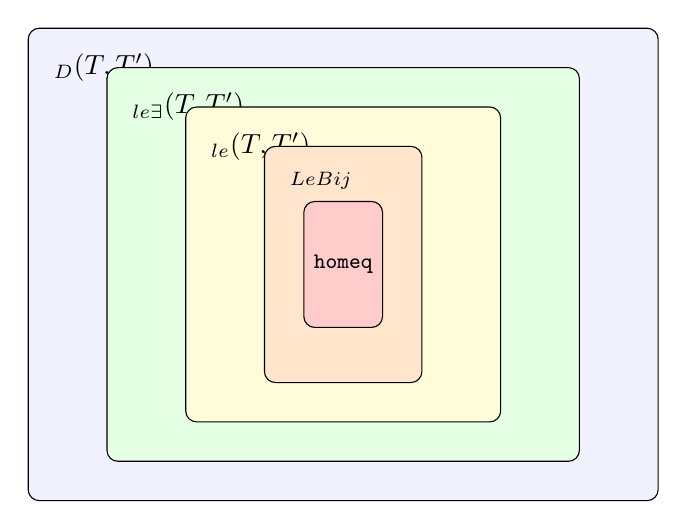
\begin{tikzpicture}[
  set/.style={draw, ellipse, minimum width=2cm, minimum height=1cm, align=center},
]

% 集合を入れ子で描画
\draw[fill=blue!5, rounded corners] (-4,-3) rectangle (4,3);
\node[anchor=north west] at (-3.8,2.8) {$\Hom_D(T, T')$};

\draw[fill=green!10, rounded corners] (-3,-2.5) rectangle (3,2.5);
\node[anchor=north west] at (-2.8,2.3) {$\Hom_{le\exists}(T, T')$};

\draw[fill=yellow!15, rounded corners] (-2,-2) rectangle (2,2);
\node[anchor=north west] at (-1.8,1.8) {$\Hom_{le}(T, T')$};

\draw[fill=orange!20, rounded corners] (-1,-1.5) rectangle (1,1.5);
\node[anchor=north west] at (-0.8,1.3) {$\Hom_{LeBij}$};

\draw[fill=red!20, rounded corners] (-0.5,-0.8) rectangle (0.5,0.8);
\node at (0,0) {\footnotesize $\homeq$};

\end{tikzpicture}
\caption{射の集合の包含関係}
\label{fig:hom-inclusion}
\end{figure}

\subsection{関手の合成}

\begin{figure}[htbp]
\centering
\begin{tikzcd}[row sep=large, column sep=large]
\cattwo \arrow[r, "U_{minL}"] & \catlebij \arrow[r, "U_{bij}"] & \catle \arrow[r, "U_{idx}"] & \catleexists \arrow[r, "U_{mono}"] & \catD
\end{tikzcd}
\caption{忘却関手の連鎖}
\label{fig:forgetful-chain}
\end{figure}

各忘却関手が「忘れる」もの：
\begin{itemize}
  \item $U_{minL}$：minLayer 保存条件
  \item $U_{bij}$：全単射条件
  \item $U_{idx}$：$\indexMap$ のデータ性（存在に落とす）
  \item $U_{mono}$：単調性の構造（存在量化に落とす）
\end{itemize}

%=============================================================================
\section{結論}
%=============================================================================

\subsection{本稿の成果}

本稿では、構造塔理論における複数の圏論的レーン設計について体系的に解説した：

\begin{enumerate}[label=(\arabic*)]
  \item \textbf{$\catD$}：最小限の存在量化条件。確率論の可測写像に適する。
  
  \item \textbf{$\catle$}：明示的な添字写像。時刻の順序保存を表現。
  
  \item \textbf{$\catleexists$}：存在版。忘却関手の faithful 性を改善。
  
  \item \textbf{$\catlebij$}：全単射レーン。groupoid ではないことに注意。
  
  \item \textbf{$\cattwo$}：minLayer 保存。普遍性の一意性を保証。
\end{enumerate}

\subsection{Bourbaki の精神}

本設計は、Bourbaki の「必要十分な一般性」の原則を体現している：

\begin{itemize}
  \item 各レーンは、特定の応用に対して過不足のない条件を提供
  \item 忘却関手により、レーン間の関係が明示的に記述される
  \item Lean 4 による形式検証で、設計の正しさが保証される
\end{itemize}

\subsection{今後の展望}

\begin{itemize}
  \item 極限・余極限の存在条件の詳細な解析
  \item 随伴関手の構成（自由-忘却）
  \item 確率論（停止時間、マルチンゲール）への本格的応用
  \item 高次圏論への拡張
\end{itemize}

%=============================================================================
% 付録
%=============================================================================

\appendix

\section{型ラッパ一覧}

\begin{table}[htbp]
\centering
\caption{Category インスタンス衝突回避のための型ラッパ}
\begin{tabular}{lll}
\toprule
ラッパ型 & 元の型 & 用途 \\
\midrule
\texttt{TowerD\_D} & \texttt{TowerD} & $\catD$ の圏インスタンス \\
\texttt{TowerD\_LeExists} & \texttt{TowerD} & $\catleexists$ の圏インスタンス \\
\texttt{TowerD\_LeBij} & \texttt{TowerD} & $\catlebij$ の圏インスタンス \\
\bottomrule
\end{tabular}
\end{table}

\section{Sanity Check 集}

以下は各ファイルで確認されている基本的な性質（すべて \texttt{rfl} で証明可能）：

\begin{lstlisting}[caption=Sanity checks]
-- Cat_le_exists.lean
example (T : TowerD_LeExists) (x : (T : TowerD).carrier) :
    (𝟙 T : T ⟶ T).map x = x := rfl

-- Cat_le_functors.lean
example (T : TowerD) (x : T.carrier) :
    (forgetLeToD.map (𝟙 T)).map x = x := rfl

example (x : TowerD.natTowerD.carrier) :
    (forgetLeToD.map (natSuccHomLe ≫ natSuccHomLe)).map x 
      = Nat.succ (Nat.succ x) := rfl

-- Cat_LeBij.lean
example {T T' T'' : TowerD} (g : T' ⟶ₗᵇ T'') (f : T ⟶ₗᵇ T') (x : T.carrier) :
    (comp g f).map x = g.map (f.map x) := rfl

-- Cat_WithMin.lean
example (T T' T'' : TowerWithMin) (f : T ⟶ T') (g : T' ⟶ T'') :
    (f ≫ g).map = g.map ∘ f.map := rfl
\end{lstlisting}

\section{参考文献}

\begin{enumerate}
  \item Bourbaki, N. \textit{Éléments de mathématique: Théorie des ensembles}. Hermann.
  \item Mac Lane, S. \textit{Categories for the Working Mathematician}. Springer (1971).
  \item Awodey, S. \textit{Category Theory}. Oxford University Press (2010).
  \item The mathlib Community. \textit{The Lean Mathematical Library}. 
    \url{https://github.com/leanprover-community/mathlib4}
  \item Williams, D. \textit{Probability with Martingales}. Cambridge University Press.
\end{enumerate}

\end{document}
